\chapter{Исследовательская часть}
В исследовательской части будут представлено время работы реализации алгоритма и качественная оценка реалистичности преломляющих эффектов.
\section{Технические характеристики}
Тестирование выполнялось на устройстве со следующими техническими характеристиками:
\begin{itemize}
	\item Операционная система Pop!\_OS 22.04 LTS \cite{ubuntu} Linux \cite{linux};
	\item Оперативная память 16 Гб;
	\item Процессор AMD® Ryzen 7 2700 eight-core processor × 16 \cite{amd}.
\end{itemize}

Во время тестирования устройство было подключено к блоку питания и не нагружено никакими приложениями, кроме встроенных приложений окружения, окружением и системой тестирования.

\section{Оценка реалистичности преломляющих эффектов}

При одинаковых коэффициентах преломления равным 1 у жидкости и воздуха, стержень не должен иметь эффекта преломления.

На рисунке \ref{img:inter-coef} продемонстрировано, что стержень не имеет эффекта преломления в разных средах. 

\begin{figure}[ht!]
	\centering{
		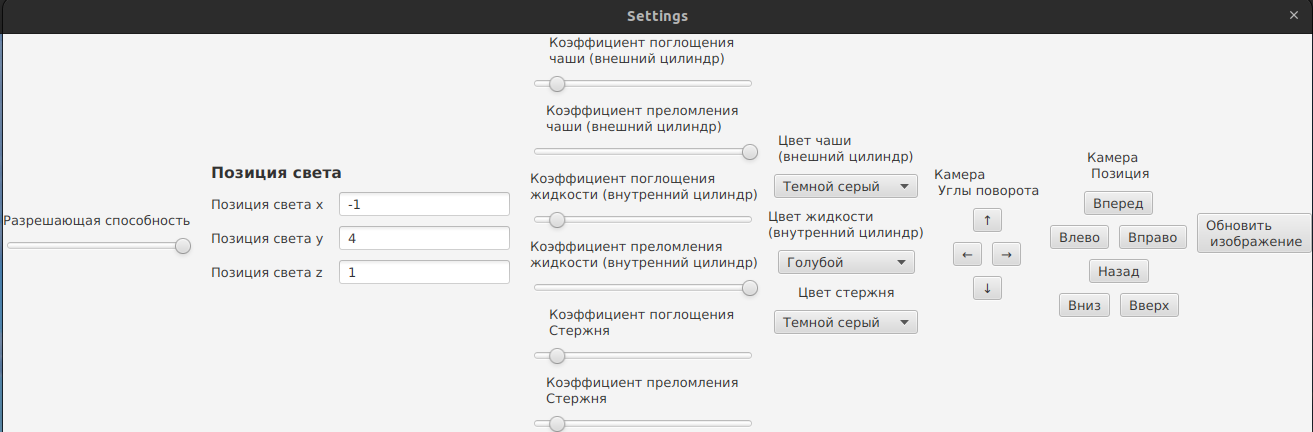
\includegraphics[width=0.8\textwidth]{assets/coef-1.png}
		\caption{Демонстрация эффекта преломления стержня, при коэффициенте преломления жидкости равного 1.}
		\label{img:inter-coef}}
\end{figure}
\FloatBarrier

На рисунке \ref{img:13-coef} демонстрируется, что при коэффициентах преломления равных 1,3 у жидкости и емкости наблюдается оптический эффект увелечения стержня между средами воздуха, емкости и жидкости.

\begin{figure}[ht!]
	\centering{
		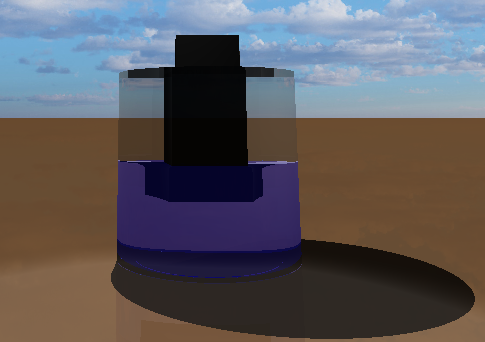
\includegraphics[width=0.8\textwidth]{assets/coef-1.3.png}
		\caption{Демонстрация эффекта преломления стержня, при коэффициенте преломления жидкости равного 1,3.}
		\label{img:13-coef}}
\end{figure}
\FloatBarrier

На рисунке \ref{img:16-coef} демонстрируется, что при коэффициентах преломления равных 1,6 и 1 у жидкости и емкости соответственно наблюдается оптический эффект увелечения стержня между средами воздуха и жидкости.

\begin{figure}[ht!]
	\centering{
		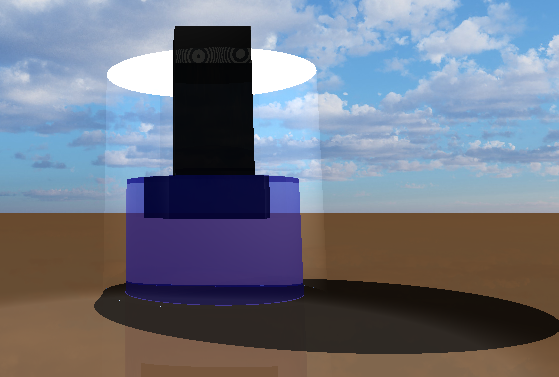
\includegraphics[width=0.8\textwidth]{assets/coef-1.6.png}
		\caption{Демонстрация эффекта преломления стержня, при коэффициенте преломления жидкости равного 1,6.}
		\label{img:16-coef}}
\end{figure}
\FloatBarrier


\section{Влияние глубины рекурсии на время создания изображения и его качество}

В алгоритме обратной трассировки лучей задается глубина рекурсии.

В таблице \ref{tab:time1} продемонстрировано пользовательское время программы при разном глубине рекурсии.

\begin{table}[ht!]
	\begin{center}
		
		\caption{Пользовательское время работы программы при разной глубине рекурсии}
		\label{tab:time1}
		\begin{tabular}{|c|c|}
			\hline
			Глубина рекурсии & Время в с. \\
			\hline
			1  & 0.779 \\
			\hline
			2  & 0.892 \\
			\hline
			3  & 1.282 \\
			\hline
			4  & 1.618 \\
			\hline
			5  & 2.081 \\
			\hline
			6  & 3.128\\
			\hline
			7  & 4.830\\
			\hline
			8  & 7.369\\
			\hline
			
		\end{tabular}
	\end{center}
\end{table}
\newpage
На рисунке \ref{graph:r} представлено время работы обратной трассировки лучей.

\begin{figure}[ht!]
	\begin{center}
		\captionsetup{singlelinecheck = false, justification=centerfirst}
		\begin{tikzpicture}
			\begin{axis}[
				xlabel={глубина рекурсии},
				ylabel={время, с},
				width = 0.95\textwidth,
				height=0.3\textheight,
				xmin=0, xmax=9,
				legend pos=north west,
				xmajorgrids=true,
				grid style=dashed,
				]
				\addplot[
				blue,
				semithick,
				mark = x,
				mark size = 3pt,
				thick,
				] file {assets/time.dat};
				
				
				\legend{
					Обратная трассировка лучей
				}
			\end{axis}
		\end{tikzpicture}
		\centering
		\caption{Результаты времени работы обратной трассировки лучей}
		\label{graph:r}
	\end{center}
\end{figure}

На рисунках \ref{img:deep-1}, \ref{img:deep-3}, \ref{img:deep-5} демонстрируются изображения, которые выдает программа при глубине рекурсии: один, три и пять соответственно. 

\begin{figure}[ht!]
	\centering{
		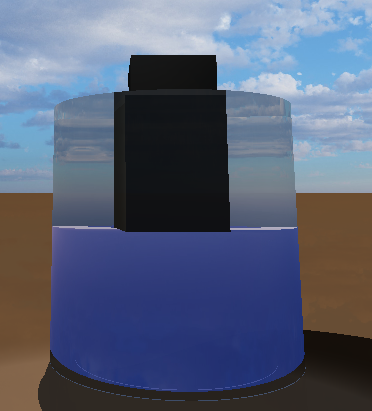
\includegraphics[width=0.5\textwidth]{assets/deep-1.png}
		\caption{Изображение при глубине рекурсии равным 1}
		\label{img:deep-1}}
\end{figure}
\FloatBarrier
\begin{figure}[ht!]
	\centering{
		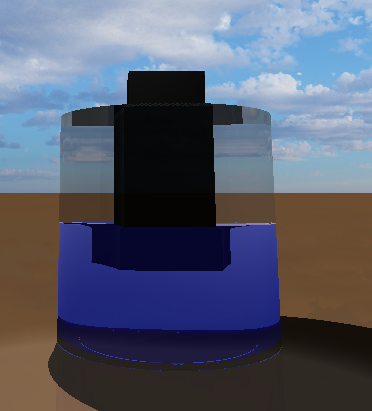
\includegraphics[width=0.5\textwidth]{assets/deep-3.png}
		\caption{Изображение при глубине рекурсии равным 3}
		\label{img:deep-3}}
\end{figure}
\FloatBarrier
\begin{figure}[ht!]
	\centering{
		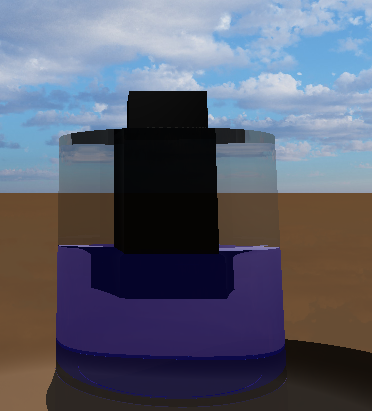
\includegraphics[width=0.5\textwidth]{assets/deep-5.png}
		\caption{Изображение при глубине рекурсии равным 5}
		\label{img:deep-5}}
\end{figure}
\FloatBarrier
\newpage

Как видно из графика \ref{graph:r}, при глубине рекурсии больше пяти время растет значительно относительно предыдущих шагов, при этом при глубине рекурсии больше трех \ref{img:deep-3}, \ref{img:deep-5} изображение почти не изменяется. 

\section*{Вывод}

В результате было выявлено, что реализация алгоритма соответствует реальному преломлению, представлено время работы реализации алгоритма и показано, что глубина рекурсии 3 является оптимальной по времени и выдает изображение соответствующе реальному преломлению.